\chapter{Binary Collatz Tree}
\label{ch:binary_tree}

\section{\texorpdfstring{Transforming $H_{C,3}$ into a binary tree}{Transforming HC3 into a binary tree}}
A binary tree is a rooted tree, where each node has at most two immediate successors. Those nodes, from which no edge goes out downward, are called leaves, the others are called internal nodes. In a full binary tree, all internal nodes have exactly two children \cite[p.~102]{Ref_Higham_2015}. Full binary trees have an odd number $2n+1$ of nodes. Of these $n+1$ are leaves and $n$ are inner nodes \cite[p.~134]{Ref_Kersting_Wakolbinger_2008}. Each node in a binary tree has a left subtree and a right subtree, which is why a binary tree is inherently recursive, since the left and right subtrees of the root are themselves binary trees \cite[p.~246-247]{Ref_Mazur_2010}. As it often pops up in combinatorial problems, the famous $n$-th Catalan number, named after the Belgian mathematician Eugène Catalan, comes in connection with binary trees into play. For $n\ge1$ it specifies the number of binary trees on $n$ vertices \cite[p.~247]{Ref_Mazur_2010}:
\[
B_n=\sum_{i=0}^{n-1}B_iB_{n-1-i}=\sum_{i=1}^{n}B_{i-1}B_{n-i}=\frac{1}{n+1}\binom{2n}{n}
\]

There is an interesting property that trees exhibit regarding abstract algebra. Let's have a look at the algebraic structure of magmas. Consider an element $x$ of a magma $(M,*)$ which is an iterated product of other elements in $M$. Such an element can be described by a planar (no edges cross each other) rooted binary tree whose $n$ leaves are labelled by these other elements $x_1,\ldots,x_n\in M$ \cite[p.~96]{Ref_Kalka_2016}.

Binary trees make well-suited data structures for storing information. With about $2^n$ data points, a search of a binary tree takes only about $n$ steps, compared to about $2^{n-1}$ steps to search a
simple list \cite[p.~84]{Ref_Benjamin_2009}.

Jan Kleinnijenhuis and Alissa M. Kleinnijenhuis \cite{Ref_Kleinnijenhuis} introduced a binary tree $T_{\ge0}$ that can be derived from $H_{C,3}$ in the manner described next. The edges are changed according to the following procedure: whenever a parent node $w$ has edges to its child nodes $v_0,v_1,\ldots,v_n$, on the tree $H_{C,3}$, we draw an edge from $w$ to $v_0$, and edges from $v_i$ to $v_{i+1}$ for each $i=1,\ldots,n-1$, in the binary new tree. Note that the nodes $v_1,v_2,\ldots,v_n$ are sorted in increasing order of label $v_0<v_1<\ldots<v_n$, which is already given by \ref{eq:n_fold_right_sibling_k}. Figure~\ref{fig:bt3} and \ref{fig:bt3_rot} display tat tree -- once in our standard layout and once reversed (from bottom to top).

\begin{figure}[H]
	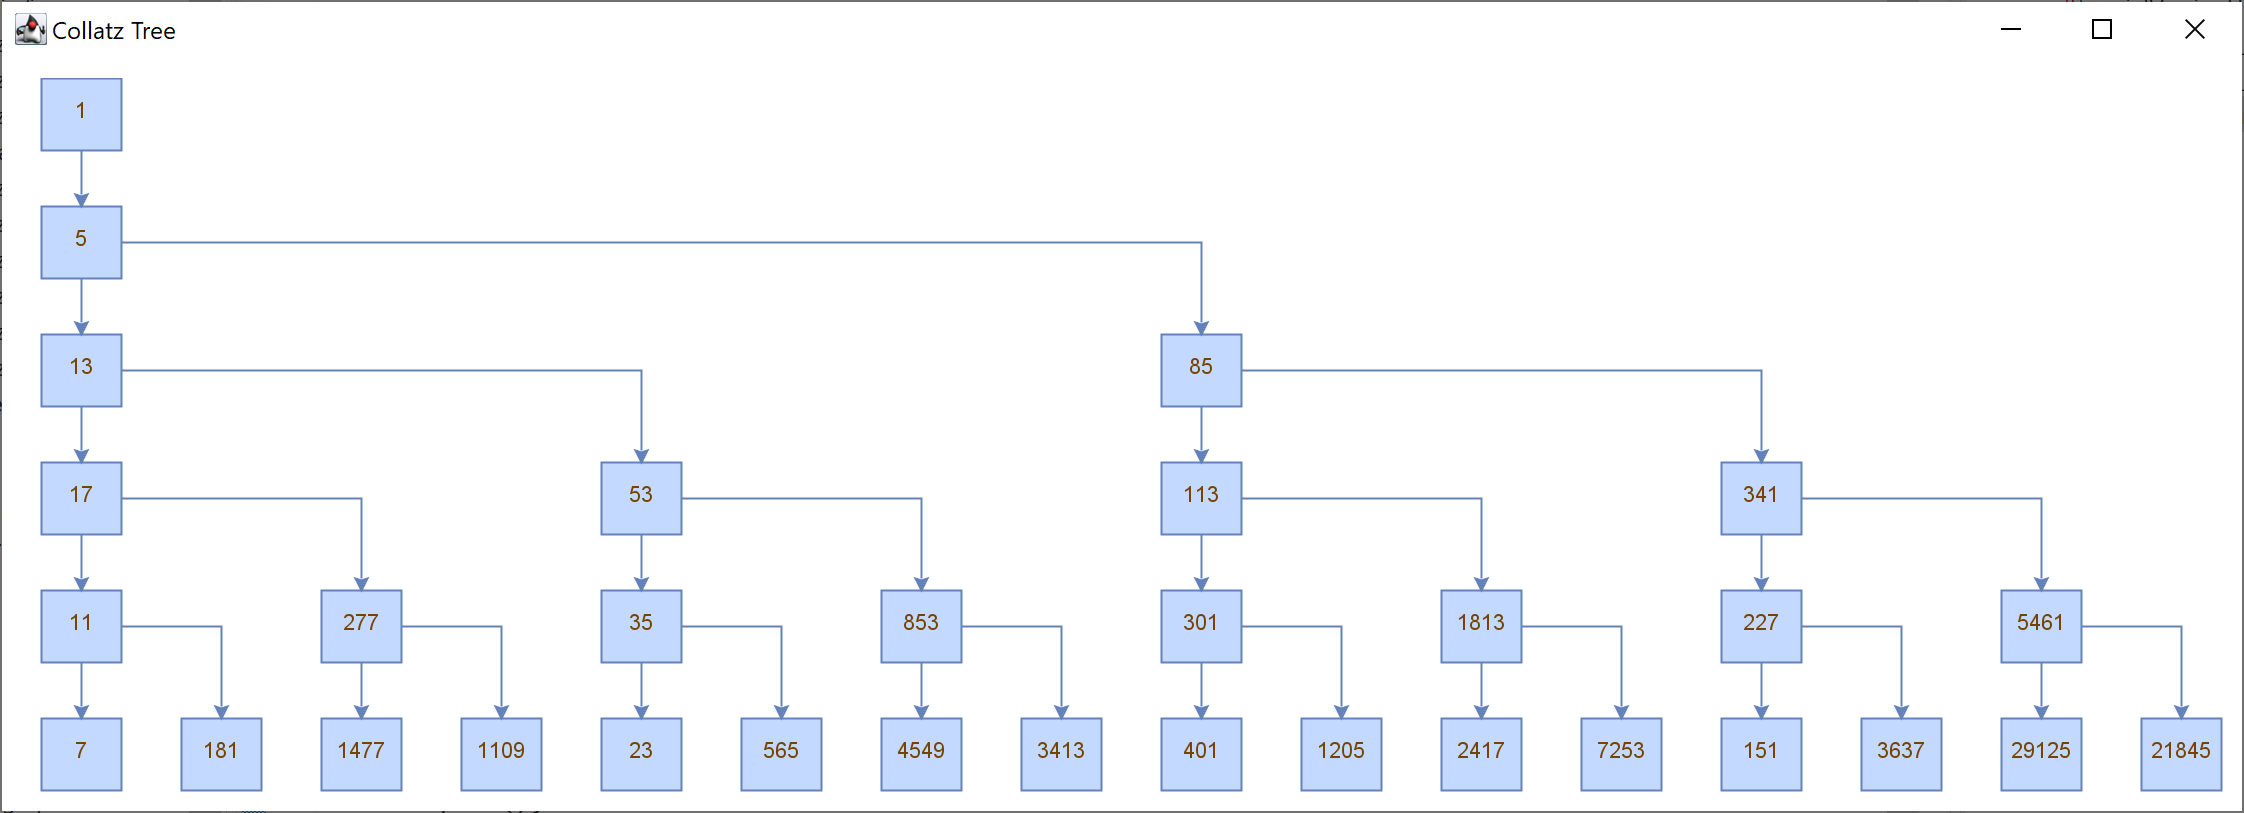
\includegraphics[width=1.00\textwidth]{figures/bt_3.png}
	\caption{The Collatz Tree transformed to the binary tree $T_{\ge0}$}
	\label{fig:bt3}
\end{figure}

\begin{figure}[H]
	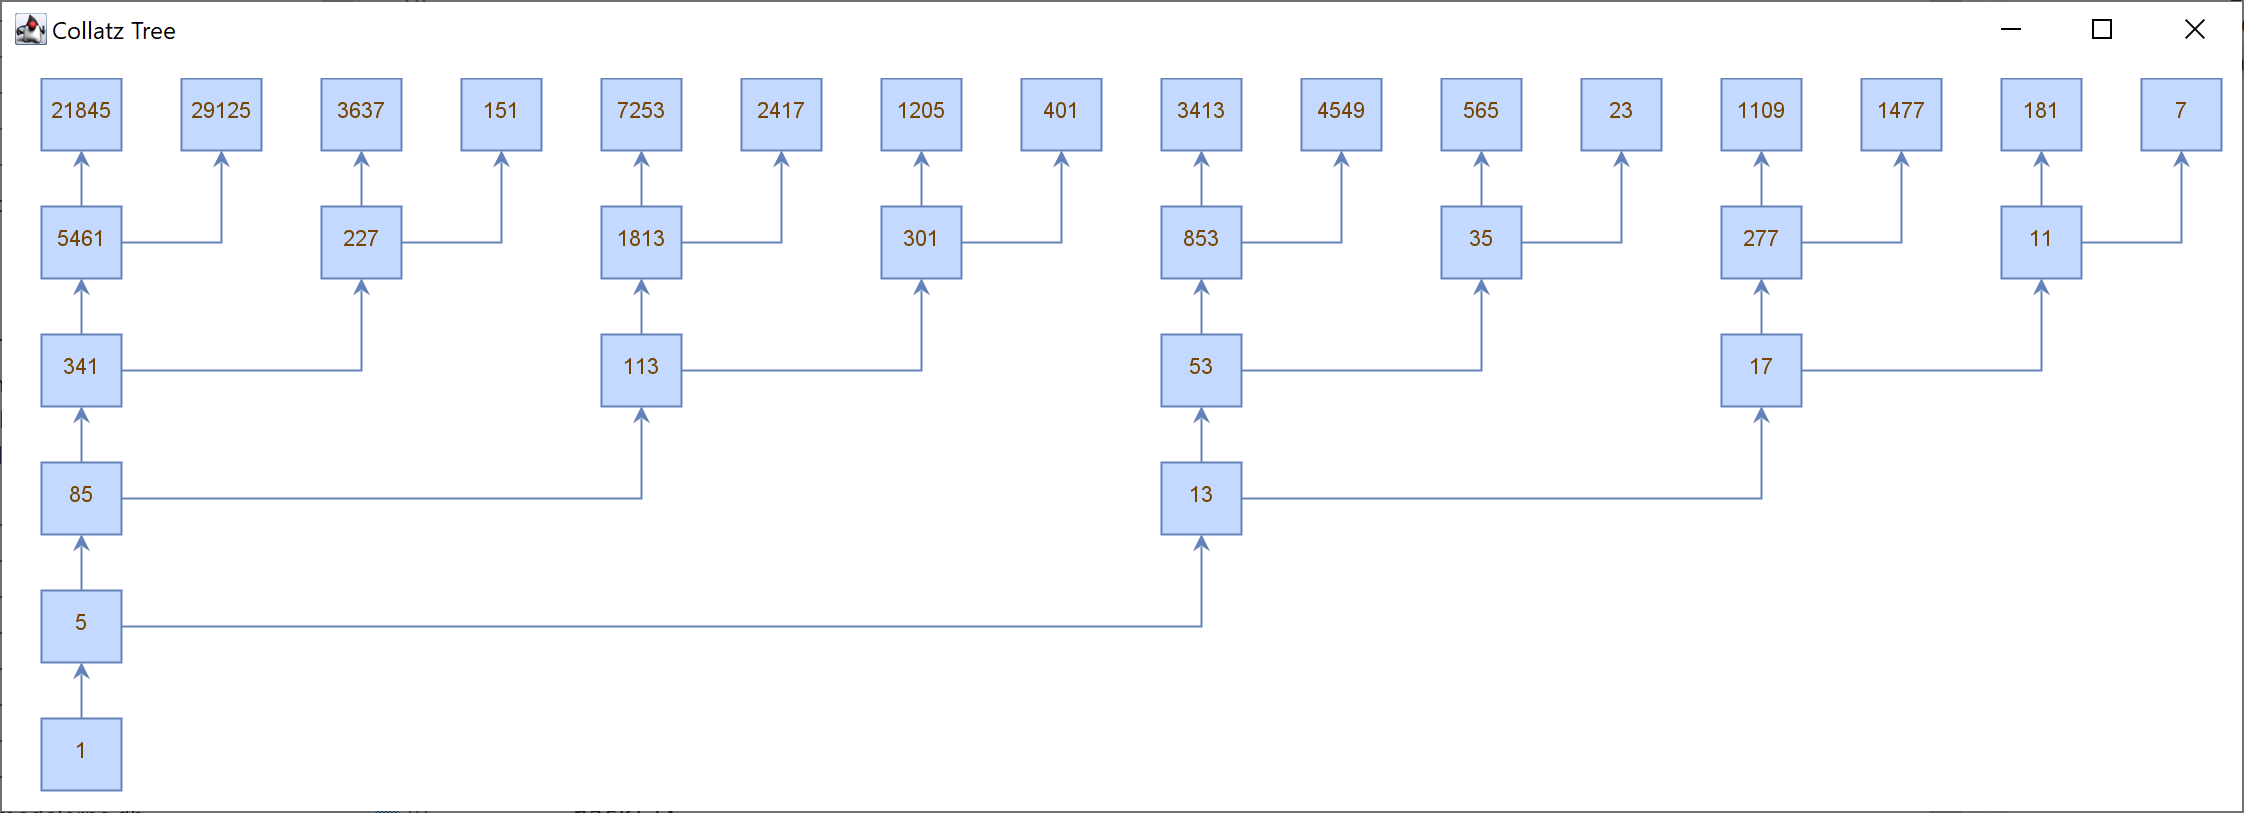
\includegraphics[width=1.00\textwidth]{figures/bt_3_rot.png}
	\caption{The binary tree $T_{\ge0}$ with \textit{bottom-to-top} layout orientation}
	\label{fig:bt3_rot}
\end{figure}

For navigating within this binary tree, Jan Kleinnijenhuis and Alissa M. Kleinnijenhuis \cite{Ref_Kleinnijenhuis} defined an Upward function $U(n)$ and a Rightward function $R(n)$ as follows:

\begin{equation}
\label{eq:bintree_3_rightward_upward}
\setlength{\arraycolsep}{1.6em}
\begin{array}{cc}
U(n)=\begin{cases}
        4n+1	&	n\equiv 1\pmod 6\\
        16n+5	&	n\equiv 5\pmod 6
    \end{cases} &
R(n)=\begin{cases}
    \nicefrac{(2^2n-1)}{3}	&	n\equiv 1\pmod{18}\\
    \nicefrac{(2^3n-1)}{3}	&	n\equiv 5\pmod{18}\\
    \nicefrac{(2^4n-1)}{3}	&	n\equiv 7\pmod{18}\\
    \nicefrac{(2^1n-1)}{3}	&	n\equiv 11\pmod{18}\\
    \nicefrac{(2^2n-1)}{3}	&	n\equiv 13\pmod{18}\\
    \nicefrac{(2^1n-1)}{3}	&	n\equiv 17\pmod{18}
\end{cases}
\end{array}
\end{equation}

The Upward function's domain consists of the two residue classes $[1]_6,[5]_6$, which form the multiplicative (cyclic) group $\mathbb{Z}^\ast_6=\{1,5\}=<5>$. Consequently, this domain excludes all integers divisible by $2$ and $3$, which is due to the fact that this binary tree (just like our tree $H_{C,3}$) does not contain even numbers and additionally all leaves -- namely those nodes labeled with an integer divisible by three -- were deleted. The function $U(n)$ is very similar to the function~\ref{eq:next_sibling_k3} and to the more general function~\ref{eq:n_fold_right_sibling_k} (when setting $n=1,k=3$) which both calculate the right-sibling of a given vertex. This is clear, since siblings in $H_{C,3}$ are successors within the binary tree. In the end, for a node $v_0$ having a leaf as right-sibling in $H_{C,3}$, the function $U(n)$ is defined as $v_1=4v_0+1$ executed twice $v_1=4(4v_0+1)+1=16v_0+5$, because we must skip this leaf -- all leafs are deleted from the binary tree without exception.

Jan and Alissa M. Kleinnijenhuis \cite{Ref_Kleinnijenhuis} moreover defined $S_{\ge0}=\mathbb{Z}^\ast_6$ as the multiplicative group modulo $6$ and $S_{-1}=\mathbb{Z}/6\mathbb{Z}\setminus\mathbb{Z}^\ast_6=\{0,2,3,4\}$ as the set of all non-invertible elements (non-units) of $\mathbb{Z}/6\mathbb{Z}$. The set $N(T_C)=N(H_{C,3})=S_{-1}\cup S_0\cup S_1\cup S_2\ldots$ contains the labels of all nodes $v_n$, to which a path from the root in $H_U$ exists, in other words, this set contains all integers $n$ for which the orbit of $n$ under the (uncompressed) Collatz function~\ref{eq:func_collatz} converges to $1$.

The set $S_{\ge1}=N(T_C)\setminus(S_{-1}\cup S_{0})=\bigcup_{j=1}^{\infty}S_j$ is the union of all sets $S_j$ for $j\ge1$. And generalized $S_{\ge j}=\bigcup_{i=j}^{\infty}S_i$. In order to comprehend this, we first have to get behind how the sets $S_j$ are structured and why they form a partition of the union sets $S_{\ge j}$. For instance, $S_0\cup S_1\cup S_2\ldots$ is a partition of $\mathbb{Z}^\ast_6$.

The set $S_0$ consists of all nodes resulting as output of $R(n)$ within the binary tree $T_{\ge0}$, which means that $S_0$ is the codomain of the function $R(n)$ operating on nodes within $T_{\ge0}$.

The binary tree $T_{\ge0}$ can be transformed to a (pruned) binary tree $T_{\ge1}$. For this, we first identify the pruning candidates -- they are all nodes $v\in S_0$ that lie in the Rightward function's codomain. Then let $v_0,v_1,v_2,v_3$ be nodes in $T_{\ge0}$, whereas $v_1=R(v_0)$ and $v_2=U(v_0)$ and $v_3=U(v_1)$. Then we delete $v_1$ including its incoming edge from $v_0$ and its outgoing edge to $v_3$. The node $v_3$ we first reconnect with an incoming edge from $v_2$ and then identify it as pruning candidate for a later transformation of the pruned tree $T_{\ge1}$ to a more pruned tree $T_{\ge2}$.

The set $S_1$ contains all nodes that are (as per description above) identified as pruning candidate for the next transformation of $T_{\ge1}$ to $T_{\ge2}$. After having transformed $T_{\ge1}$ to $T_{\ge2}$, the more pruned binary tree $T_{\ge2}$ contains nodes that are identified as pruning candidates for another upcoming transformation of $T_{\ge2}$ to $T_{\ge3}$ -- these nodes are elements of the set $S_2$. This pruning algorithm is repeatedly applied in the same pattern. And in this way we obtain the sets $S_1,S_2,S_3,\ldots$ and so forth. Finally for the sets apply $S_j=\{n\mid U^{-j}(n)\in S_0\}$

The idea behind transforming the Collatz tree into a binary tree is that binary trees exhibit special properties, which make them easier to handle and due to iteratively pruning them one may show that all odd numbers are covered by the Collatz tree.

I have an interesting additional challenge (I know you solved this arithmetically) - but let us take a viewpoint from group theory:

The (cyclic) multiplicative group $(\mathbb{Z}/18\mathbb{Z})^\times=\mathbb{Z}^\ast_{18}=\{1,5,7,11,13,17\}=<5>$ has an order $ord(\mathbb{Z}^\ast_{18})=6$ and based on Euler's theorem we can derive the following congruences from $5^j5^{6n+6-j}\equiv1\pmod{18}$:

\[
\begin{array}{cc}
j=0 & [1]_{18}\cdot5^{6n+6}\equiv1\pmod{18}\\
j=1 & [5]_{18}\cdot5^{6n+5}\equiv1\pmod{18}\\
j=2 & [7]_{18}\cdot5^{6n+4}\equiv1\pmod{18}\\
j=3 & [17]_{18}\cdot5^{6n+3}\equiv1\pmod{18}\\
j=4 & [13]_{18}\cdot5^{6n+2}\equiv1\pmod{18}\\
j=5 & [11]_{18}\cdot5^{6n+1}\equiv1\pmod{18}
\end{array}
\]

Now let us consider the following congruences:

\[
\begin{array}{cc}
&[1]_{18}\cdot4\equiv1\pmod{3}\\
&[5]_{18}\cdot8\equiv1\pmod{3}\\
&[7]_{18}\cdot16\equiv1\pmod{3}\\
&[17]_{18}\cdot2\equiv1\pmod{3}\\
&[13]_{18}\cdot4\equiv1\pmod{3}\\
&[11]_{18}\cdot2\equiv1\pmod{3}
\end{array}
\]

Having in mind that, if $m\mid n$ (in our case $3\mid18$) the map $r\bmod n \rightarrow r\bmod m$ is a homomorphism $(\mathbb{Z}/n\mathbb{Z})^\times\rightarrow(\mathbb{Z}/m\mathbb{Z})^\times$, what is the morphism between both congruences shown above - the one $\bmod{18}$ and the other one $\bmod3$?


